\documentclass[10pt,a4paper]{article}
\usepackage[margin=2cm]{geometry}
\usepackage{libertinus}
\usepackage[T1]{fontenc}
\usepackage{microtype}
\usepackage{amsmath}
\usepackage{graphicx}
\usepackage{booktabs}
\usepackage{caption}
\usepackage{enumitem}
\usepackage{xcolor}
\usepackage[section]{placeins}
\usepackage[hidelinks]{hyperref}

\definecolor{maxorange}{HTML}{eb6834}
\definecolor{ringblue}{HTML}{2a78d6}
\newcommand{\maxs}{\textcolor{maxorange}{\textbf{strongest bin}}}
\newcommand{\ring}{\textcolor{ringblue}{\textbf{ring search}}}
\captionsetup{font=small,labelfont=bf}
\setlist{itemsep=1pt,topsep=3pt}
\graphicspath{{../figures/}}

\title{A ring search for the megarena's carriers\\[2pt]
\large The library's global pipeline with its strongest-bin peak search and
with a ring search, on fmac renders of megarenas}
\author{Vernier team}
\date{\today}

\begin{document}
\maketitle

\begin{abstract}
\noindent
The megarena detector starts by finding the pattern's two carriers in the
spectrum of the whole picture. Today \texttt{PatternPhase::peaksSearch} takes
the \maxs{} of the spectrum, then the strongest bin in another direction. This
note adds a second search, the \ring, which judges every bin against the bins
at the same distance from the centre, and compares the two inside the
library's own global pipeline: one FFT, one Gaussian band-pass per carrier,
phase planes, then the megarena code. Nothing else changes. Four megarenas are
rendered by fmac, the Vernier project's marker renderer, at 44 poses, and
each picture is spoiled four ways: 704 pictures. On each, both searches run;
the carriers they demodulate are compared with the true ones, and the decoded
position with the true one.
\end{abstract}

\section*{Key findings}

\begin{itemize}
  \item \textbf{The \ring{} finds the right carriers twice as often}: 414 of
        704 pictures against 196. On every picture where the \maxs{} found
        them, the \ring{} found them too.
  \item \textbf{The decoded position gains less}: right on 155 pictures against
        99, 1.6 times as often. The global pipeline itself is now the limit.
  \item \textbf{Square on, the two are level.} Both find the right carriers on
        all 24 clean square-on views, and over the four conditions both decode
        64 of 96 square-on pictures at the right position.
  \item \textbf{At 15° of tilt the \ring{} doubles the right positions} (44
        against 22 of 96 pictures); the \maxs{} often takes the megarena
        code's own line, at a third of the carrier, for a carrier.
  \item \textbf{From 30° the global pipeline fails whatever the carriers.}
        The \ring{} still finds the right pair on 60 of 96 pictures at 30°,
        but only 6 decode at the right position, and none at 50°: a single
        band-pass cannot follow a carrier whose frequency changes across the
        picture.
  \item \textbf{The detector never says it failed.} \texttt{patternFound()}
        was true on all 1\,408 runs, including the 1\,154 decoded at a wrong
        position, 1\,135 of them three periods or more away.
\end{itemize}

\textbf{In short:} the \ring{} is a safe change for the global pipeline. It
never loses the carriers the \maxs{} finds, and decodes more pictures. But on
its own it does not make the global pipeline work on tilted views: that needs
a measurement that follows the carriers across the picture, and a decoder that
can tell a wrong code from a right one.

\section{The two searches}

\paragraph{The \maxs} (\texttt{PatternPhase::peaksSearch}, unchanged). Take the
magnitude of the picture's spectrum. Keep the bins between 20 and 500 from the
centre, blur them over 3$\times$3 and keep half the plane. The strongest bin is
the first carrier. Cut a thin wedge around its direction (its width set by the
band-pass $\sigma = 3$) and the opposite one; the strongest bin left is the
second carrier.

\paragraph{The \ring} (\texttt{PatternPhase::ringPeaksSearch}, new). In plain
words:
\begin{itemize}
  \item \textbf{It fades the picture to zero at its edges} (a Hann window,
        after taking the mean out) before its own FFT, so the picture's
        border does not draw a bright cross through the spectrum.
  \item \textbf{It sums each bin with its 8 neighbours}, so a carrier spread
        over a few bins still counts in full.
  \item \textbf{It scores each bin against its ring}: its value over the mean
        of all bins at the same distance from the centre, one bin wide. Edges,
        shadows and clutter put their energy at low frequencies, but evenly
        around the ring, so they score low; a carrier is a narrow spike and
        scores high. A ring quieter than the average one is held to the
        average.
  \item \textbf{It keeps every local maximum that scores at least 0.2 of the
        best}, from 6 bins out (counted along the picture's short side) to
        0.35 cycles per pixel, strongest first.
  \item \textbf{It knows the code's line.} If the spectrum at three times a
        peak is more than half as strong as the peak, the peak is the
        megarena code's line at a third of the carrier, and the carrier is
        taken at three times it.
  \item \textbf{It looks for the second carrier where it can be}: 0.7 to 1.4
        times the first one's distance from the centre and at least 60° away.
\end{itemize}
The first peak that has such a partner gives the pair. Both are put back in
the upper half plane and ordered as \texttt{peaksSearch} orders them, so the
rest of the pipeline is the same. It is switched on with
\texttt{detector.setBool("ringPeakSearch", true)}; the default stays the
\maxs. It runs on the CPU path only; the CUDA engine keeps its own search.
Figure~\ref{fig:spectrum} shows both on the same board.

\begin{figure}[h]
\centering
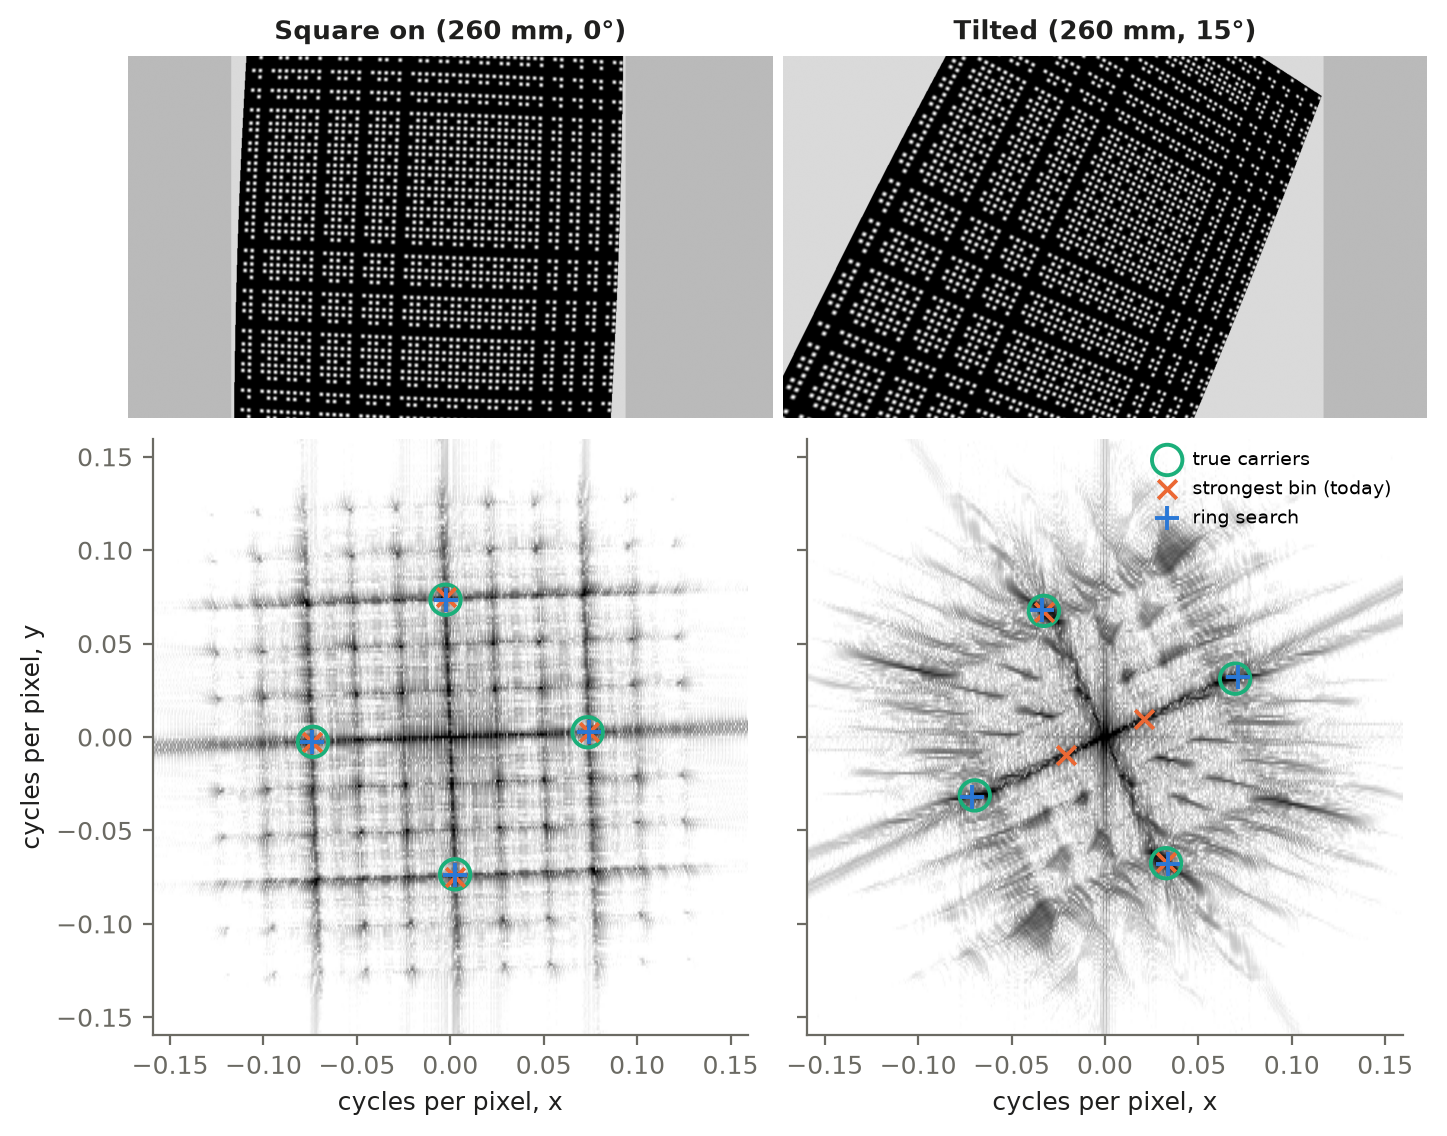
\includegraphics[width=\linewidth]{spectrum.png}
\caption{The 3.54\,mm megarena at 260\,mm, square on (left) and tilted by 15°
(right), and the middle of each picture's spectrum, with the bins each search
picked. Square on, both pick the true carriers. Tilted, the \maxs{} takes the
code's line at a third of one carrier, close to the centre; the \ring{} stays
on the carriers.}
\label{fig:spectrum}
\end{figure}

\section{The setup}

\paragraph{The pictures.} fmac renders through a thin-lens camera: a 6\,mm
lens at f/2 on 6\,µm pixels, focused at 300\,mm, 1280$\times$720,
$f_x = f_y = 1000$\,px, with lens distortion, diffraction and the Rec.~709
transfer curve, 8-bit output, undone back to linear intensities. The four
megarenas are 280$\times$200\,mm, with dot pitches of 2.5, 3.54, 5 and
7.07\,mm and a code of order 6. Each is rendered at 44 poses: 20 tilted
20--40° and placed around the frame, 260--380\,mm off; and 24 test views at
220 to 450\,mm, square on and tilted by 15, 30 and 50°.

\paragraph{What is added.} Each picture is used four ways: as rendered;
with Gaussian noise of $\sigma = 0.03$; with three hard-edged \emph{shadows},
rectangles of a fifth to three fifths of the frame darkened to 40--80\,\%; and
with a \emph{blind}, a strong stripe pattern of 8--24\,px period at a random
angle covering a third of the frame's width. That makes 704 pictures.

\paragraph{What is counted.} The detector is
\texttt{MegarenaPatternDetector} with the pitch as its period and code size 6,
everything else at its defaults. Per picture and search:
\begin{itemize}
  \item \emph{Right carrier pair}: the gradients of the two fitted phase
        planes, the carriers actually demodulated, both lie within 20\,\% of
        the true carriers. The true carriers come from the true pose, at the
        board point seen at the middle of the picture.
  \item \emph{Right position}: the decoded $(x, y)$ lies within half a period
        of the true one on both axes. The detector reports minus the board
        point under the picture's centre, 15 periods off on both axes,
        modulo the code's length of 189 periods; that relation was read off
        the clean square-on views and holds to a hundredth of a period on
        every board. A misread code lands a whole code bit or more away:
        of all 1\,408 decodes, 254 are within half a period, 19 between half
        a period and three, and 1\,135 three periods or more away.
\end{itemize}

\section{Results}

\subsection{Overall}

\begin{figure}[h]
\centering
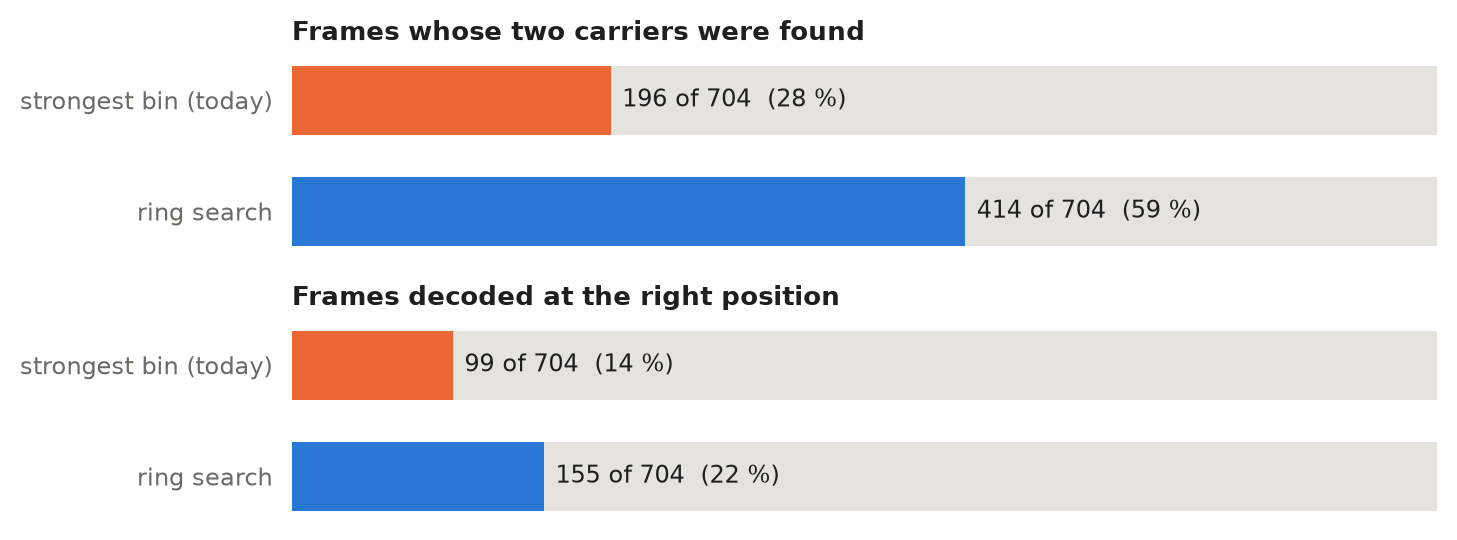
\includegraphics[width=\linewidth]{overall.png}
\caption{Every picture: 4 boards, 44 poses, 4 conditions. The grey track is
all 704.}
\label{fig:overall}
\end{figure}

Figure~\ref{fig:overall}. The \ring{} finds the right carriers on 414 pictures
against 196, and never misses a pair the \maxs{} found. The right position
follows less: 155 pictures against 99. The \ring{} decodes 69 pictures the
\maxs{} does not, and loses 13 it does.

Those 13 are not wrong carriers: on 12 of them both searches found the right
pair. The two searches sometimes place the same carrier one bin apart, the
\ring{} on the maximum of its 3$\times$3 sum, the \maxs{} on its lightly
blurred maximum. The band-pass then sits one bin apart, the phase maps differ
slightly, and the code reading, which samples the dots through those maps, can
flip: on one clean view at 400\,mm the decoded $y$ moved by 108 periods for a
one-bin shift of the other carrier. Over the 196 pictures where both found
the right pair, this goes the \ring's way: right position with both on 86,
with the \ring{} only on 32, with the \maxs{} only on 12.

\subsection{Square on against tilted}

\begin{figure}[h]
\centering
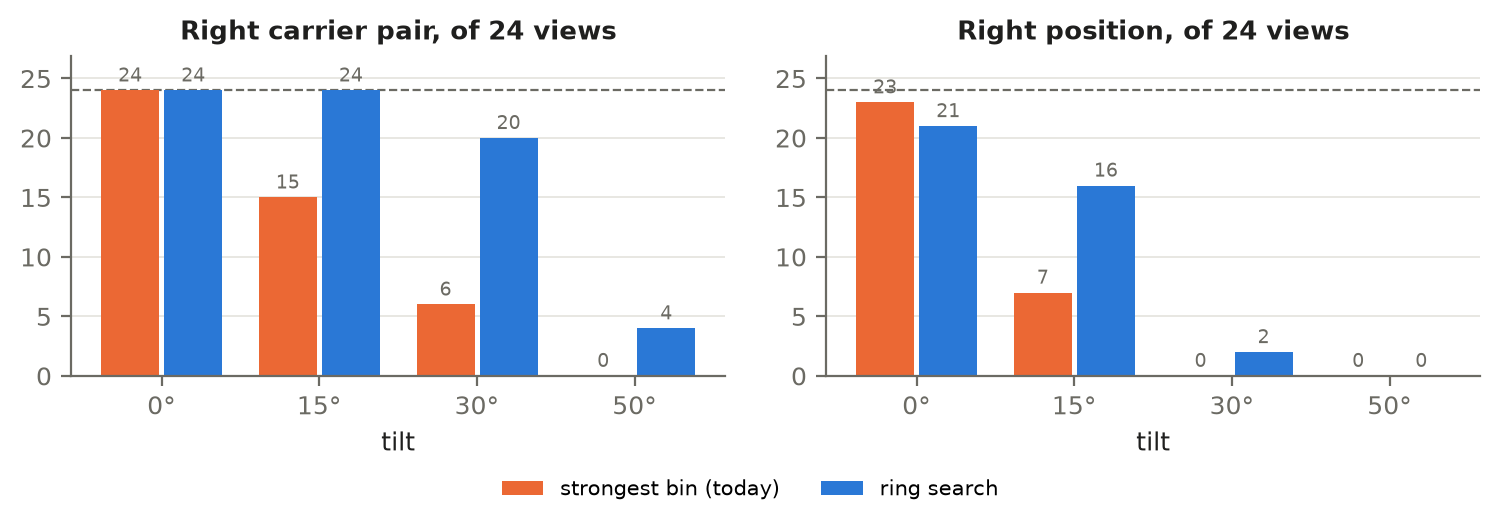
\includegraphics[width=\linewidth]{tilt.png}
\caption{The 24 clean test views by tilt: four boards, six distances from 220
to 450\,mm at each tilt. The dashed line is every view.}
\label{fig:tilt}
\end{figure}

Figure~\ref{fig:tilt}. Square on, both searches find the right carriers on
every view and the right position on nearly every one (23 and 21; over the four
conditions, 64 and 64 of 96). At 15° the \maxs{} finds the right pair on 15
views of 24, the \ring{} on all 24, and the right positions follow: 7 against
16 (22 against 44 of 96 over the four conditions). At 30° the \ring{} still
finds 20 right pairs, but only 2 views decode at the right position; at 50°,
none with either search. The calibration views, all tilted 20--40°, say the
same: right pairs 60 against 189 of 320, right positions 11 against 41.

\subsection{Noise, shadows and a blind}

\begin{figure}[h]
\centering
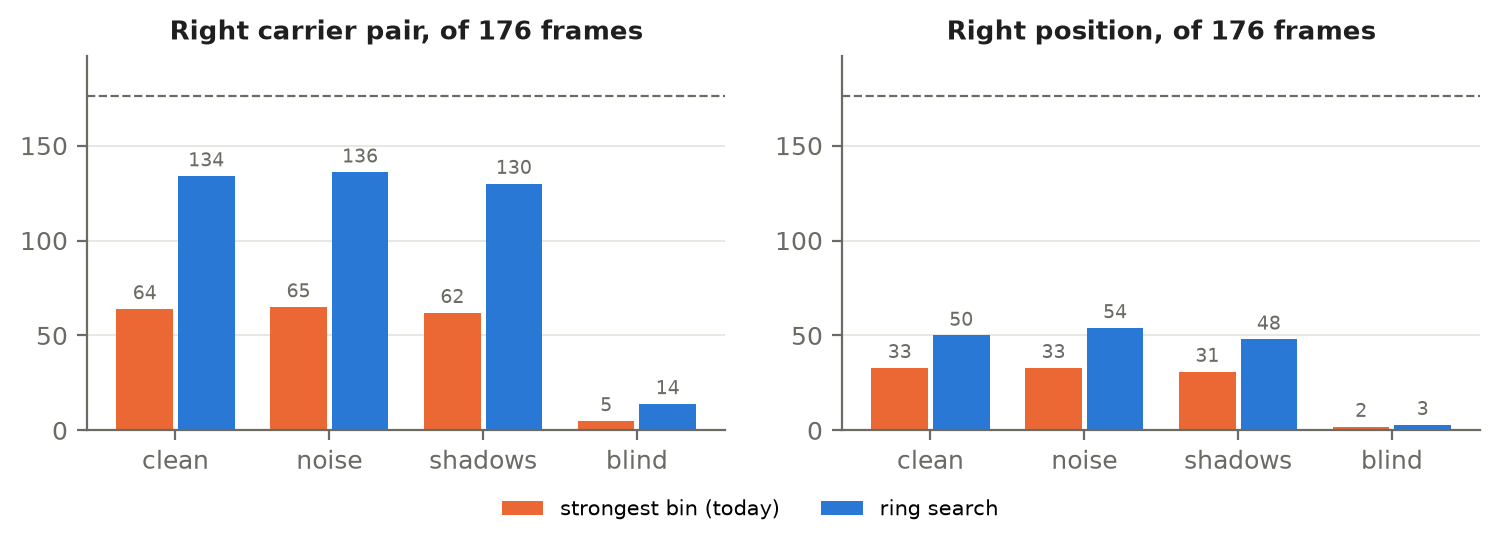
\includegraphics[width=\linewidth]{conditions.png}
\caption{Every picture, by what was added: as rendered, Gaussian noise of
$\sigma = 0.03$, three hard-edged shadows, a blind over a third of the
frame.}
\label{fig:conditions}
\end{figure}

Figure~\ref{fig:conditions}. Noise and shadows change almost nothing for
either search. The blind's stripes are the strongest thing in the picture
and both searches take them for a carrier on most of its pictures: 5 and 14
right pairs of 176, 2 and 3 right positions. Getting past it would take
trying more than one pair, which needs a decoder that says when a code is
wrong.

\section{Why the gain is smaller in the global pipeline}

\paragraph{One band-pass for the whole picture.} The pipeline isolates each
carrier with one Gaussian band-pass of $\sigma = 3$ bins and fits one phase
plane to the whole picture. Square on, the carrier has one frequency
everywhere and this is exact. Tilted, the dot spacing changes across the
picture, the carrier spreads over more bins than the band-pass keeps, and the
phase is no longer a plane. The \ring{} finds the carriers on 259 pictures
where the position is still wrong, against 98 for the \maxs; all but 12 of
the 259 are tilted views.

\paragraph{No failure signal.} \texttt{findCodePosition} returns the best match
of the sequence read, whether or not it truly matches, and
\texttt{patternFound()} only checks that two peaks were found. So a misread
code comes out as a confident position far from the truth, and the detector
cannot fall back to its next candidate pair. Both would help any peak search.

\section{What to take from this}

\begin{itemize}
  \item The \ring{} is a safe improvement to the carrier search: square on it
        changes nothing on average, and elsewhere it finds the carriers twice
        as often and never loses a pair the \maxs{} finds. It costs one more
        FFT of the picture.
  \item On its own it does not make tilted views work in the global pipeline.
        The next steps are a measurement that follows the carriers across the
        picture, and a code check that rejects a sequence not found in the
        code, so that a wrong decode is reported, and the next candidate pair
        tried.
  \item The code reading is sensitive to where the band-pass is centred: one
        bin can change the decoded position by many periods. Worth a look on
        its own.
  \item Caveats: one renderer, one camera, one board size, fixed poses; the
        noise, shadows and blind were added to the renders, not photographed.
        The CUDA backend was not changed.
\end{itemize}

\section*{Appendix: reproducing}

The comparison is the \texttt{comparingPeakSearch} example, which runs both
searches of \texttt{MegarenaPatternDetector} on every picture listed in a CSV
file. \texttt{truth.csv} lists the 704 pictures with their pitch, the true
board point under the picture's centre and the true carriers; the pictures
are 16-bit PNG with linear intensities. With a build of the library and its
examples, run from the repository's root:

\begin{verbatim}
doc/ring-peak-search/run.sh <build-dir> <picture-dir>
\end{verbatim}

\noindent It writes \texttt{results.csv}, one row per picture and search with
the pose, the phase planes and the peaks; scores it against the truth with
\texttt{analyse.py} into \texttt{scored.csv}; draws the figures with
\texttt{plot.py} and builds this PDF. About 11 minutes on 12 cores.

\end{document}
